\clearpage

\lehead[]{\sf\hspace*{-2.00cm}\textcolor{white}{\colorbox{lightblue}{\parbox[c][0.70cm][b]{1.60cm}{
\makebox[1.60cm][r]{\thechapter}\\ \makebox[1.60cm][r]{ÜBUNG}}}}\hspace{0.17cm}\textcolor{lightblue}{\chaptertitle}}
\rohead[]{\textcolor{lightblue}{\chaptertitle}\sf\hspace*{0.17cm}\textcolor{white}{\colorbox{lightblue}{\parbox[c][0.70cm][b]{1.60cm}{\thechapter\\
ÜBUNG}}}\hspace{-2.00cm}}
%\chead[]{}
\rehead[]{\textcolor{lightblue}{AvHG, Inf, My}}
\lohead[]{\textcolor{lightblue}{AvHG, Inf, My}}

\section{Mausereignisse -- Übungen}

\subsection{Aufgabe 1: Markierungen setzen}

Wenn der Benutzer mit der Maus in das Fenster klickt, wird die Stelle, auf die
er geklickt hat, mit einem kleinen roten Kreis markiert. Wenn der Benutzer
einen Doppelklick macht, wird statt eines Kreises ein Quadrat gezeichnet.

Anmerkung: Da der Bildschirmhintergrund vor dem Zeichnen gelöscht wird, ist
immer nur eine Markierung zur Zeit sichtbar.


\subsection{Aufgabe 2: Zeichenbrett}

Es soll eine Art „Zeichenbrett“ programmiert werden.

\begin{center}
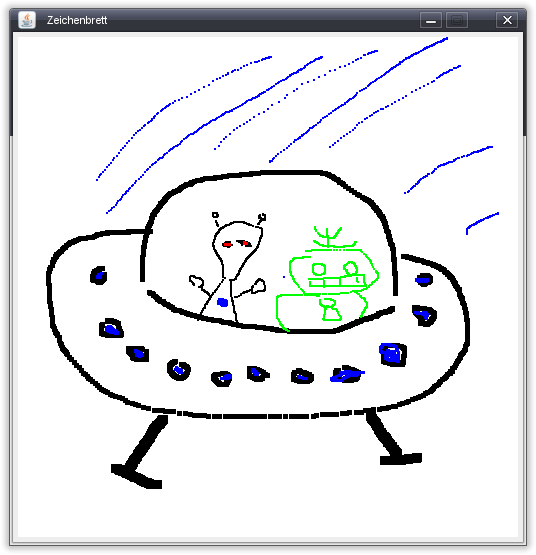
\includegraphics[width=0.5\textwidth]{./inf/SEKII/22_Java_Mausereignisse/Zeichenbrett.png}
\end{center}

\begin{compactenum}[a)]
\item Erzeuge dazu ein Frame mit einem weißen Hintergrund. Wenn der Benutzer
mit der Maus in das Fenster klickt, wird das Pixel an der Stelle, auf die
geklickt wurde, schwarz gezeichnet (Anmerkung: mit der
\myClass{Graphics}-Methode \lstinline|drawLine()| kann man auch Punkte
zeichnen). Wenn man mit der gedrückten Maus über das Fenster fährt, werden
ebenfalls alle Pixel, über die die Maus fährt, schwarz eingefärbt. Alle „alten“
Punkte, die der Benutzer zuvor gezeichnet hat, sollen immer wieder mit
gezeichnet werden. Das Programm muss sich also die Farbe aller Pixel merken.
Lege dazu ein zweidimensionales Array vom Typ \myClass{Color} an, das in seiner
Größe der Breite und Höhe des Fensters entspricht. Nachdem du das Array erzeugt
hast, haben alle Einträge zu Beginn den Wert \lstinline|null| („kein
Color-Objekt vorhanden“). Wenn der Benutzer einen Punkt anklickt, erhält der
entsprechende Eintrag im Array die Farbe \lstinline|Color.BLACK| zugewiesen. Da
der Hintergrund weiß ist, brauchen beim Zeichnen nur die Pixel tatsächlich
gemalt werden, bei denen der Array-Eintrag ungleich \lstinline|null| ist. Wenn
man jedes Mal alle Pixel neu malen würde, würde das das System zeitlich zu sehr
belasten.

\item Wenn der Benutzer ein kleines oder großes ’L’ drückt, wird das bisher
gezeichnete Bild gelöscht und der Bildschirm ist wieder weiß. Setze dazu alle
Einträge im Array auf den Wert \lstinline|null| zurück.

\item Erweitere das Zeichenbrett so, dass man auch farbige Zeichnungen machen
kann. Der Benutzer kann die Farbe des Zeichenstiftes über die Tastatur
verstellen, z.B:

’r’ oder ’R’: rot

’b’ oder ’B’: blau

’g’ oder ’G’: grün

’s’ oder ’S’: schwarz

Zu Beginn ist die Farbe schwarz ausgewählt. 

\item Über die Tasten ’1’ bis ’9’ kann man die Stift-Breite einstellen. Bei
einem Maus-Klick wird immer ein rechteckiges Kästchen mit der angegebenen
Breite eingefärbt, bei einer Stiftbreite von 4 werden zum Beispiel 4*4 Pixel
gefärbt.

In der Methode \lstinline|keyTyped()| kann man die Stiftbreite mit folgendem
Code-Auszug geschickt einstellen:

\begin{lstlisting}
if (e.getKeyChar() >= '1' && e.getKeyChar() <= '9') {
    breite = e.getKeyChar() - '0';
}
\end{lstlisting}

Dieser Code nutzt die Tatsache aus, dass die Buchstaben von ’0’ bis ’9’ in der
Zeichentabelle fortlaufende ASCII-Codes besitzen. ’0’ wird durch die Zahl 48
kodiert, ’1’ durch die Zahl 49, \ldots\ ’9’ durch die Zahl 57.
\end{compactenum}


\subsection{Aufgabe 3: Ameisen fangen}

Grundidee: Im Anwendungsfenster wird an irgendeiner zufällig ausgewählten
(festen) Position eine Ameise angezeigt, die der Benutzer möglichst schnell
durch einen Mausklick einfangen muss. Wenn er die Ameise getroffen hat,
verschwindet sie und eine andere Ameise wird an anderer, zufällig ausgewählter
Stelle angezeigt. Der Benutzer muss in einer vorgegebenen Zeitspanne (zum
Beispiel 15 Sekunden) möglichst viele Ameisen fangen. Damit die Anwendung
interessanter wird, gibt es acht verschiedene Ameisenbilder, von denen immer
eines zufällig ausgewählt wird. Die Ameisenbilder findest du im Kursrepository.
Alle Ameisenbilder sind 13 Pixel breit und 13 Pixel hoch.

Im Konstruktor der Anwendung werden alle acht Ameisenbilder in ein Array
geladen. Während des Spiels wird immer nur eine Ameise an einer zufälligen
Position angezeigt. Ein Objekt der Klasse \myClass{Timer} wird gestartet, um den
Zeitablauf überprüfen zu können. Die abgelaufene Zeit wird im Programm durch
Zählen der \lstinline|myPaint()|-Aufrufe ermittelt. Wenn die Zeitspanne
abgelaufen ist, wird dem Benutzer in der \lstinline|myPaint()|-Methode mit
\lstinline|drawString()| angezeigt, wie viele Ameisen er fangen konnte.

Hinweis: Neben dem Anwendungsfenster braucht keine weitere Klasse programmiert
werden.


\subsection{Aufgabe 4: Das Lampenproblem}

Im Anwendungsfenster wird eine Reihe von Lampen positioniert. Der Benutzer hat
die Aufgabe, die Lampen auszuschalten. Wenn er eine Lampe anklickt, wird jedoch
nicht die Lampe selber an- oder ausgeschaltet, sondern es werden die beiden
Nachbarlampen umgeschaltet.

Wenn der Benutzer im abgebildeten Beispiel die zweite Lampe von links anklickt,
geht die erste Lampe aus und die dritte Lampe geht an. Die zweite Lampe selber
verändert sich nicht.

Wenn der Benutzer eine der Lampen am Rand anklickt, wird nur der eine Nachbar
verändert, den die Lampe hat. Klickt man im abgebildeten Beispiel die erste
Lampe, geht die zweite Lampe aus.

\begin{center}
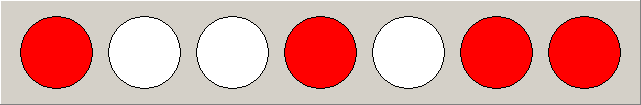
\includegraphics[width=0.4\textwidth]{./inf/SEKII/22_Java_Mausereignisse/Lampenproblem.png}
\end{center}

Gehe folgendermaßen vor:

\begin{compactenum}[a)]
\item Vor einiger Zeit haben wir im Unterricht eine Klasse \myClass{Lampe}
programmiert. Erzeuge ein neues Anwendungsfenster mit einem Array von sieben
Lampen, die wie abgebildet nebeneinander positioniert werden. Zu Beginn sind
alle Lampen ausgeschaltet.

\item Fange im Anwendungsfenster die Mausereignisse ab. Wenn der Benutzer mit
der Maus in das Fenster klickt, muss die Nummer der angeklickten Lampe
ermittelt werden. Gehe dazu in einer Schleife alle Lampen durch und vergleiche
die Mausposition mit der Position der Lampe. Eine Lampe wird „getroffen“, wenn
sich die x-Position der Maus zwischen der linken Seite der Lampe (x-Position
Maus >= x-Position Lampe) und der rechten Seite der Lampe (x-Position Maus <=
x-Position Lampe + Breite der Lampe) befinden. Außerdem muss die y-Position der
Maus zwischen der oberen und der unteren Seite der Lampe liegen. Merke dir in
einer Variablen, welche Lampe angeklickt wurde. Es kann auch sein, dass der
Benutzer gar keine Lampe getroffen hat. Dann sollte die Variable einen
ungültigen Wert haben, zum Beispiel -1. Gib den Wert der Variable zum Test auf
der Konsole aus, damit du weißt, ob das Programm die getroffene Lampe richtig
ermittelt.

\item Wenn eine Lampe getroffen wurde, wird der Zustand der Nachbarlampen
verändert (von an auf aus oder umgekehrt) und anschließend wird das Fenster neu
gezeichnet. Beachte, dass die Rand-Lampen nur einen Nachbarn besitzen.
\end{compactenum}


\subsection{Aufgabe 5: Game of Life erweitern}

\begin{compactenum}[a)]
\item Erweitere das \emph{Game of Life} so, dass man im angehaltenen Zustand den
Zustand einer Zelle verändern kann (von lebendig zu tot oder umgekehrt) indem
man mit der Maus auf die Zelle klickt.

\item Wenn der Benutzer im angehaltenen Zustand mit der Maus über mehrere Zellen
fährt, soll der Zustand aller überfahrenen Zellen umgedreht werden. Beachte
dabei, dass sich die Maus auf ihrem Weg längere Zeit in derselben Zelle
befindet. Der Zustand der Zelle darf natürlich trotzdem nur einmal verändert
werden.
\end{compactenum}


\subsection{Aufgabe 6: Snake}

Du sollst den Spiele-Klassiker \emph{Snake} programmieren.

\begin{center}
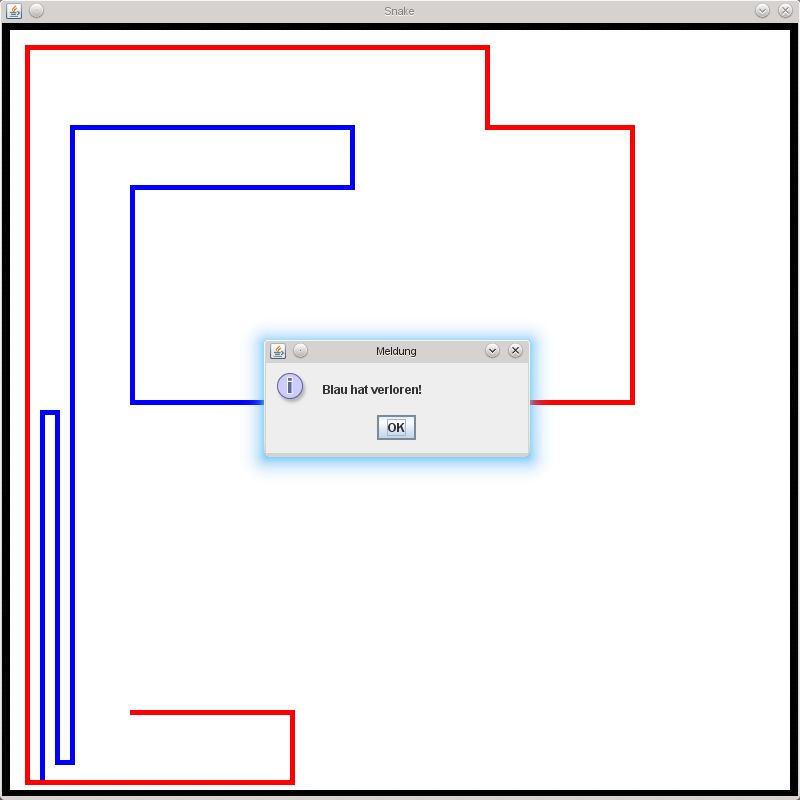
\includegraphics[width=0.75\textwidth]{./inf/SEKII/22_Java_Mausereignisse/Snake.png}
\end{center}

\begin{compactenum}[a)]
\item Erzeuge ein Anwendungsfenster mit Höhe und Breite von je 800 Pixeln. Das
Spielfeld besteht aus einzelnen Punkten (Koordinaten), die jeweils ein Quadrat
von 5x5 Pixeln auf dem Bildschirm darstellen. 160X160 Punkte füllen somit das
Anwendungsfenster von 800x800 Pixeln komplett aus. Das Spielfeld sollst du als
zweidimensionales Integer-Array anlegen. In den einzelnen Array-Elementen
kannst du für dann für jeden Punkt des Spielfeldes den Zustand speichern:

	0: Dieser Punkt ist noch frei.	
	
	1: Dieser Punkt wird vom Körper der roten Schlange belegt.	
	
	2: Dieser Punkt wird vom Körper der blauen Schlange belegt.	
	
	-1: Dieser Punkt ist Teil der Wand	

Im Konstruktor der Klasse solltest du das Array so initialisieren, dass die
beiden äußeren Reihen an jeder Seite die Mauer bilden.

In der Mitte des Spielfeldes sollte der Kopf der roten Schlange und direkt
links daneben der Kopf der blauen Schlange sein. Setze die Geschwindigkeit in
x-Richtung für die rote Schlange auf 1 und für die blaue Schlange auf -1.
Speichere die x- und y-Position sowie die x-und y-Komponenten der
Geschwindigkeit von beiden Schlangen in geeigneten Variablen.

\item In der \lstinline|myPaint()|-Methode werden zunächst auf Basis der
aktuellen Koordinaten und Geschwindigkeiten die neuen x- und y-Positionen der
beiden Schlangenköpfe berechnet und anschließend mit entsprechenden Werten im
Spielfeld-Array markiert.

Anschließend muss die \lstinline|myPaint()|-Methode das Spielfeld zeichnen,
indem sie für alle Elemente des Arrays überprüft ob und in welcher Farbe ein
kleines Quadrat von 5x5 Pixeln gezeichnet werden soll. Die Wand wird schwarz,
die blaue Schlange blau (Wunder über Wunder) und die rote Schlange rot
gezeichnet.

Damit tatsächlich Bewegung in die Sache kommt muss jetzt nur noch ein Timer
gestartet werden. Starte ihn so, dass \lstinline|myPaint()| alle 50
Millisekunden aufgerufen wird.

\item Wenn du bis hierher alles richtig gemacht hast, werden die beiden
Schlangen beim Programmstart in entgegengesetzte Richtungen los laufen. Rot
nach rechts und blau nach links.

Erweitere das Programm jetzt so, dass die beiden Schlangen das nächste Feld nur
dann besetzen, wenn dieses zuvor noch frei war. Sollte dies bei einer von
beiden Schlangen nicht der Fall sein, sollst du die Geschwindigkeiten in x- und
y-Richtung von beiden Schlangen auf 0 setzen und den Timer stoppen.

Anschließend sollst die Spieler über eine MessageBox informieren, welcher
Spieler verloren hat (oder wenn es dir lieber ist: welcher Spieler gewonnen
hat). Siehe Abbildung.

Sobald diese MessageBox von den Spielern geschlossen wird, soll das Programm
mit \lstinline|System.exit(0)| beendet werden.

\item Jetzt fehlt noch die (für den Spielspaß nicht ganz unwesentliche)
Möglichkeit für die beiden Spieler ihre Schlangen auch tatsächlich zu steuern.

Die rote Schlange soll durch die Tastatur gesteuert werden. Welche Tasten du
für die vier Richtungen (oben, unten, rechts und links)  wählst bleibt dir
überlassen. Beachte, dass man immer nur abbiegen kann. Es ist also
beispielsweise nicht möglich direkt umzukehren (und somit Selbstmord zu
begehen). Auch kann man nicht seine Geschwindigkeit erhöhen, indem man die
aktuelle Richtung noch einmal bestätigt. Wenn der Benutzer solch unmöglichen
Steuerbefehle gibt sollen diese einfach ignoriert werden.

\item Die blaue Schlange soll mit der Maus gesteuert werden. Dabei soll aber
auch eine andere Logik benutzt werden als bei der Tastatursteuerung für die
rote Schlange. Während dort immer absolut nach oben, unten, rechts oder links
gesteuert wurde, soll der zweite Spieler seine blaue Schlange immer relativ zur
aktuellen Bewegungsrichtung beeinflussen: Rechter Mausklick führt zu einer
Drehung um 90° im Uhrzeigersinn und linker Mausklick zu einer Drehung um 90°
gegen den Uhrzeigersinn.
\end{compactenum}